\documentclass{beamer}
\usetheme{AnnArbor}
\usecolortheme{spruce}
\usepackage{circuitikz}
\usepackage{graphicx}

\title{Adders, Encoders, and Decoders}
\subtitle{More sophisticated applications of circuits}
\author[A Praveen \& A Krishnan]{Akilesh Praveen \& Ashwath Krishnan}
\institute{UMD}
\date{\today}



\begin{document}

    % title page
    \begin{frame}
        \titlepage
    \end{frame}
    
    % table of contents
    \begin{frame}
        \frametitle{Agenda}
        \tableofcontents
    \end{frame}
    
    \section{Announcements}
    
        \begin{frame}
                \vfill
                \centering
                \begin{beamercolorbox}[sep=8pt,center,shadow=true,rounded=true]{title}
                    \usebeamerfont{title}Announcements\par%
                \end{beamercolorbox}
                \vfill
             \end{frame}
    
        \subsection{Project 2}
        
            
            
            \begin{frame}
                \frametitle{Project 2}
                \begin{itemize}
                    \item Project 2 has been released, and can be found on the course website under 'Week 3' on the calendar.
                    \item Everything you need to complete the project will be covered in today's lecture, with optional supplementary material provided on the course website under Week 3's resources section.
                    
                \end{itemize}
            \end{frame}
            
            \begin{frame}
            	\frametitle{Some Reminders}
            	\begin{itemize}
            		\item As the projects become more involved, we'd like to remind you to reach out and attend office hours if you are struggling.
                    \item Additionally, here's a reminder that all projects can be group projects, but you'll have to let us know \textbf{4 days} prior to the project's due date if you'll be working in a group. (Max size of 3)
            	\end{itemize}
            	
            \end{frame}
        
    \section{Adders}
    
    	\begin{frame}
                \vfill
                \centering
                \begin{beamercolorbox}[sep=8pt,center,shadow=true,rounded=true]{title}
                    \usebeamerfont{title}Adders\par%
                \end{beamercolorbox}
                \vfill
             \end{frame}
    
    	\subsection{Addition}
    
    	\begin{frame}
    		\frametitle{Addition}
    		\begin{center}
    			{\Large How would you add the following binary numbers?}
    			\linebreak
    			{\Large \texttt{11101} \& \texttt{11011}}
    		\end{center}
    	\end{frame}
    	
    	\begin{frame}
    		\frametitle{Addition}
    		\begin{itemize}
    			\item Let's visualize the computation as long addition
    			\item How would you go about solving it this way?
			\end{itemize}
			
			\centering
			{\LARGE
			\begin{tabular}{c@{\,}c@{\,}c@{\,}c@{\,}c@{\,}c@{\,}c}
					   & 1 & 1 & 1 & 0 & 1 \\
					 + & 1 & 1 & 0 & 1 & 1 \\
					\hline
					
			\end{tabular}}
		\end{frame}
		
		\begin{frame}
    		\frametitle{Addition}
    		\begin{itemize}
    			\item Let's visualize the computation as long addition
    			\item How would you go about solving it this way?
			\end{itemize}
			
			\centering
			{\LARGE
			\begin{tabular}{c@{\,}c@{\,}c@{\,}c@{\,}c@{\,}c@{\,}c}
					   &   &   &   & {\color{red}1} &   \\
					   & 1 & 1 & 1 & 0 & 1 \\
					 + & 1 & 1 & 0 & 1 & 1 \\
					\hline
					   &   &   &   &   & 0
					
			\end{tabular}}
			
			\begin{itemize}
				\item This phenomenon is known as a {\color{red}carry}
				\item This occurs when the numbers we are adding exceed the limit imposed by the number system we are using
				\item Where else during this computation would this phenomenon occur?
			\end{itemize}
		\end{frame}	
		
		\subsection{Half Adders}
		
		\begin{frame}
			\frametitle{Half Adders}
			\begin{itemize}
				\item First, let's represent the \texttt{1}s as \texttt{TRUE}s and the \texttt{0}s as \texttt{FALSE}s
				\item Think back to last week when we talked about designing circuits that dealt with booleans
				\item The big question: can we perform the addition process that we just talked about using such gates?
				\item The answer: \textbf{absolutely}
			\end{itemize}
		\end{frame}
		
		\begin{frame}
			\frametitle{Half Adders}
			\begin{itemize}
				\item Let's take this step by step.
				\item Looking at the addition example, what's the simplest operation we can take away from that?
				\item Let's see if we can build something that can take two one-bit numbers and add them, producing a carry if applicable
				\begin{itemize}
					\item In terms of inputs, we will need two booleans
					\item In terms of outputs, we will need two booleans (one for our sum, and one for the carry)
				\end{itemize}
				\item Incidentally, we have been describing a \textbf{Half Adder}
				\item We have defined our inputs and outputs- try to design a Half Adder using the gates we've learned
			\end{itemize}
			
				
		\end{frame}
		
		\begin{frame}
			\frametitle{Half Adders}
			\begin{itemize}
				\item Below is the formal truth table and circuit diagram for an optimal Half-Adder
				\item In this case, we can see that the Sum and Carry can be represented by an \texttt{XOR} and \texttt{AND} gate, respectively \linebreak
			\end{itemize}
			\centering
			\begin{columns}
				\column{0.5\textwidth}
					\centering
					\begin{tabular}{ |p{0.75cm}||p{0.75cm}||p{0.75cm}|}
                    	 \hline
                     	\multicolumn{3}{|c|}{Half Adder} \\
                     	\hline
                     	In & Sum & Carry\\
                     	\hline
                     	0 0 & 0 & 0\\
                     	0 1 & 1 & 0\\
                     	1 0 & 1 & 0\\
                     	1 1 & 0 & 1\\
                    	 \hline
                	\end{tabular}
				
				\column{0.5\textwidth}
					\centering
					
					% HALF ADDER
					
					\begin{circuitikz} \draw
                    (-1.5,2.22) node[](b) {B}
                    (-1.5,2.78) node[](a) {A}
                    
                    (1.5,2.5) node[xor port] (myxor) {}
                    (1.5,1) node[and port] (myand) {}
                    
                    (-0.25,2.78) node[circ] (circ1) {}
                    (-0.5,2.22) node[circ] (circ2) {}
                    
                    (2.25,2.5) node[] (S) {SUM}
                    (2.35, 1) node[] (C) {CARRY}
                    
                    
                    (a) -| (myxor.in 1) 
                    (a) -| (circ1) 
                    (b) -| (myxor.in 2)
                    (b) -| (circ2)
                    (-0.25,2.78) -- (-0.25,1.28) -- (0.25,1.28)
                    (-0.5,2.22) -- (-0.5,0.72) -- (0.25,0.72);
                    
                    \end{circuitikz}
				
				
			\end{columns}
		\end{frame}

		\subsection{Full Adders}	
		
		\begin{frame}
			\frametitle{Full Adders}
			\begin{itemize}
				\item The Half Adder is great, but limited in functionality
				\item Let's work on 'scaling' it for use with multi-digit addition.
				\item How do we accomplish such a task?
				\item All we need to do is create a circuit that can:
				\begin{itemize}
					\item Add two one-bit numbers and produce a sum and carry
					\item In case the previous addition resulted in a carry, be able to add in that third number as well
				\end{itemize}
				\item Essentially, we need a logical circuit that can add three one-bit numbers. We can then use this circuit for each digit in our addition.
			\end{itemize}
		\end{frame}
		
		\begin{frame}
			\frametitle{Full Adders}
			\begin{itemize}
				\item Below is a full adder that meets our previously outlined specifications exactly.
			\end{itemize}
			
			\centering
			\begin{circuitikz}
			\draw
			(3,0) node[xor port] (myxor) {} to
			(7,0) node[xor port,anchor=in 2] (myxor1) {}
			(0,-2) node[and port,rotate=270] (myand) {}
			(5,-2) node[and port,rotate=270] (myand1) {}
			
			(2.5,-4) node[or port,rotate=270] (myor) {}
			(myxor.in 1) -- +(-2.5,0) node[anchor=east] (a) {A}
			(myxor.in 2) -- +(-2.5,0) node[anchor=east] (b) {B}
			(myor.out) node[anchor=north] (co) {Carry out}
			(myxor.in 2 -| myand.in 1) node[circ] {} -- (myand.in 1)
			(myxor.in 1 -| myand.in 2) node[circ] {} -- (myand.in 2)
			(myand.out) |- (myor.in 2)
			(myand1.out) |- (myor.in 1)
		
			(myand1.in 1) -- +(0,1.5) node[anchor=south] (cin) {Carry in}
			(myand1.in 1 |- myxor1.in 1) node[circ] {} -- (myxor1.in 1)
			(myxor1.in 2 -| myand1.in 2) node[circ] {} -- (myand1.in 2)
			(myxor1.out) node[anchor=west] (sum) {Sum}
			;
			\end{circuitikz}
		\end{frame}
		
		\begin{frame}
			\frametitle{Full Adders}
			\begin{itemize}
				\item However, it's important to note that there's an easier way to think about the implementation of a full adder
				\item Notice that the Half Adder already has half the functionality of the Full Adder that we need to design
				\begin{itemize}
					\item Specifically, it can add two one-bit numbers and produce a sum and carry. All we need to add is the ability to carry a bit into the addition.
				\end{itemize}
				\item That being said, let's try and employ the use of Half Adders within our Full Adder construction
			\end{itemize}
		\end{frame}
		
		\begin{frame}
			\frametitle{Full Adders}
			\begin{itemize}
				\item Take a look at this Full Adder construction, built using Half Adders.
			\end{itemize}
			\centering
			\begin{circuitikz} \draw
			(0,1.5) node[] (a) {A}
			(0,0) node[] (b) {B}
			(0,-1.5) node[] (c) {$C_{in}$}
			(8.25,0) node[] (sum) {SUM}
			(10.35,-3.28) node[] (cout) {$C_{out}$}
			
			(2.25,0.75) node[] (ha1) {HA}
			(6.25,-0.75) node[] (ha2) {HA}

			(1.25, 1.75) -- (1.25, -0.25) -- (3.25, -0.25) -- (3.25, 1.75) -- (1.25, 1.75)
			
			(0.25, 1.5) -- (1.25, 1.5)
			(0.25, 0) -- (1.25, 0) 

			(3.25, 1.5) -- (4.5, 1.5)
			(4.5,1.5) -- (4.5,0)
			(4.5,0) -- (5.25,0)
			
			(5.25,0.25) -- (7.25,0.25) -- (7.25,-1.75) -- (5.25, -1.75) -- (5.25,0.25) 
				
			(3.25, 0) -- (4, 0)
			(4,0) -- (4,-3.56)
			(4,-3.56)--(8.5,-3.56)	
			(9.75,-3.28) node[or port] (myor) {}	
			
			(0.25, -1.5) -- (3.8, -1.5)
			(3.8, -1.5) -- (3.8, -1.3)
			(3.8, -1.3) -- (4.2, -1.3)
			(4.2, -1.3) -- (4.2, -1.5)
			(4.2, -1.5) -- (5.25, -1.5)
			
			(7.25,0) -- (7.75, 0)
			(7.25,-1.5) -- (8.4, -1.5)
			(8.4, -1.5) -- (8.4, -3)
			
			;
			\end{circuitikz}
		\end{frame}
		
		\begin{frame}
			\frametitle{Full Adders}
			\begin{itemize}
				\item If full adders are better than half adders, why do we use them?
				\item During addition of any size, you may notice that there is always one addition 'operation' that will never have a 'carry in'
				\begin{itemize}
					\item This will always occur in the least significant bit
				\end{itemize}
				\item Since a half adder is fundamentally simpler than a full adder, we always use it when we can
				\item Now that we have the ability to add two one bit numbers, with or without a carried '1' coming into the addition, let's put these together (literally) and create a multiple digit adder.
			\end{itemize}
		\end{frame}
		
		
		\begin{frame}
			\frametitle{Full Adders}
			\begin{itemize}
				\item Here's an example of how we can chain adders to increase the number of bits that we can perform addition with
				\item Note that the Full Adder handling \texttt{A0} and \texttt{B0} can be replaced with a Half Adder\linebreak
			\end{itemize}
			
			
			
			\centering
			
			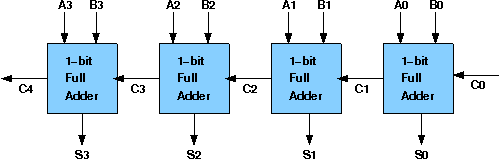
\includegraphics[width=0.8\textwidth]{4bitadder}
			
			\centering
			{\tiny Image courtesy of IIT}
			
		\end{frame}
		
		\begin{frame}
			\frametitle{Full Adders}
			
			\begin{itemize}
				\item Okay, now we can add simple n-bit numbers. But then how can computers show us numbers that aren't in binary?
				\item We need a way to translate these binary signals into numbers that we can use (or that a computer can display for us)
				\item In other words, we need to somehow convert the outputs to base-10
			\end{itemize}
			
		\end{frame}
		
		
	\section{Decoders \& Encoders}
	
		\begin{frame}
         	\vfill
         	\centering
          	\begin{beamercolorbox}[sep=8pt,center,shadow=true,rounded=true]{title}
           	\usebeamerfont{title}Decoders \& Encoders\par%
        	\end{beamercolorbox}
            \vfill
       	\end{frame}
       	
       	\subsection{Overview}
       	
       	\begin{frame}
       		\frametitle{Decoders \& Encoders}
       		\begin{itemize}
       			\item We've run into the issue of wanting to convert binary to decimal and vice versa
       			\item It turns out that this is an essential problem in digital logic (this specific case more-so in computer science)
       			\item Engineers have designed two logical circuits to accomplish these tasks
       			\begin{itemize}
       				\item Decoders are circuits that can convert binary signals into a decimal representation of those signals
       				\item Encoders are circuits that can condense those decimal representations of signals back into binary
       			\end{itemize}
       			\item These circuits can be generalized to different number systems as well, not just binary and decimal as we've specified
       		\end{itemize}
       	\end{frame}
       	
       	\subsection{Formal Definitions}
       	
       	\begin{frame}
       		\frametitle{Decoders \& Encoders}
       		\begin{itemize}
       			\item \textbf{Decoders} $ \Rightarrow $  Takes a 'denser' signal and converts it into an 'expanded' signal
       			\begin{itemize}
       				\item In our case, the decoder is converting our denser binary signal and converting it into an expanded decimal signal
       				\item Less wires coming in, more wires coming out \linebreak
       			\end{itemize}
       			
       			\item \textbf{Encoders} $ \Rightarrow $ Takes an 'expanded' signal and converts it into a 'denser' signal
       			\begin{itemize}
       				\item In our case, the encoder is converting our expanded decimal signal back into a denser binary signal
       				\item More wires coming in, less wires coming out
       			\end{itemize}
       			
       		\end{itemize}
       	\end{frame}
       	
		\subsection{Decoders}       	
       	
       	\begin{frame}
       		\frametitle{Decoders}
       		\begin{itemize}
       			\item Decoders allow us to translate a denser signal into its expanded form
       			\item Let's say we had the following 3-bit binary number below. How would you systematically go about converting it to a decimal number? \linebreak
       		\end{itemize}
       		
       		\centering
       		
       		{\LARGE \texttt{110}}
       	\end{frame}
       	
       	\begin{frame}
       		\frametitle{Decoders}
       		\begin{itemize}
       			\item The easiest way to go about this digitally is to assign a wire for each possible output
       			\item In this case, we will need 3 input wires, each representing a bit of the input binary number
       			\item Therefore, we will need 7 output wires, each representing a decimal value from 0 through 7
       			\item Given output wires $O_0$, $O_1$, ... $O_7$, let's find a way to efficiently wire 3-bit binary inputs $I_0$, $I_1$, and $I_2$ to produce those results
       		\end{itemize}
       			 
       	\end{frame}
       	
       	\begin{frame}
       		\frametitle{Decoders}
       		\begin{itemize}
       			\item Let's start with a truth table
       		\end{itemize}
       		
       		\centering
       		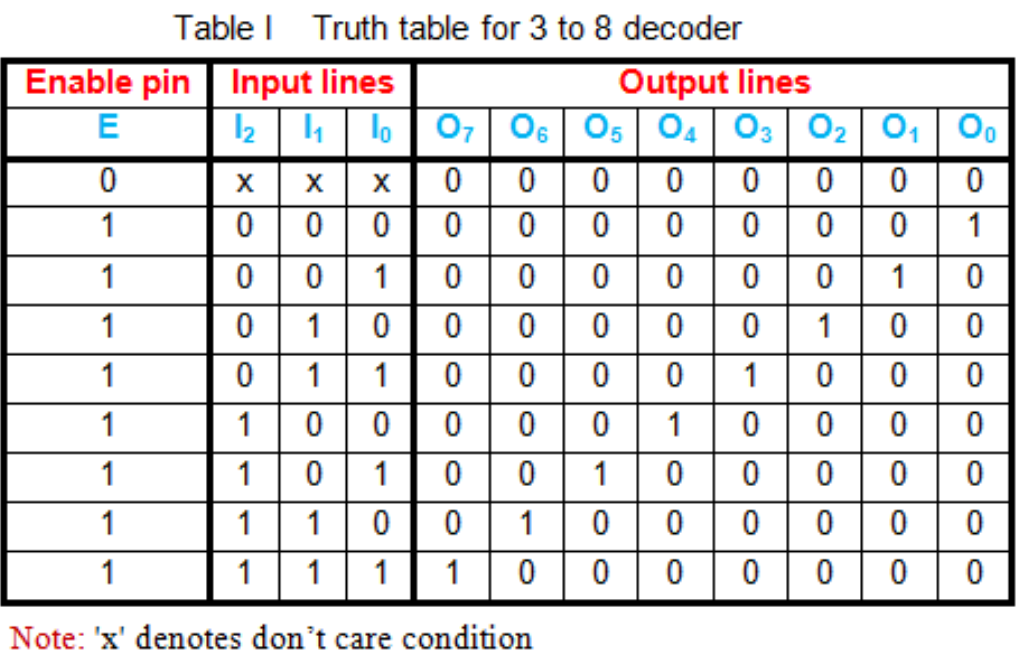
\includegraphics[width=0.8\textwidth]{decoder}
       	\end{frame}
       	
       	\begin{frame}
       		\frametitle{Decoders}
       		\begin{itemize}
       			\item It turns out, we can represent this pretty systematically
       			\item Notice the clever use of input buses, which we went over briefly last week
       		\end{itemize}
       		
       		\centering
       		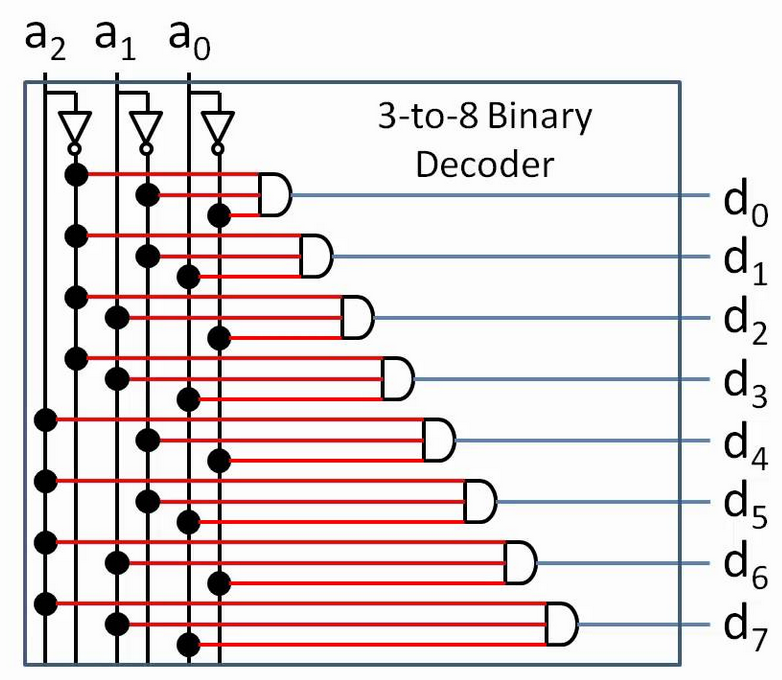
\includegraphics[width=0.5\textwidth]{decoder2}
       	\end{frame}
       	
       	\subsection{Encoders}
       	
       	\begin{frame}
       		\frametitle{Encoders}
       		\begin{itemize}
       			\item Think of encoders as the complement to decoders- they do everything a decoder can do, but backwards
       			\item Going back to our previous example, let's assume we had 7 input wires, each signifying the decimal numbers 0-7
       			\item Our goal is, based on which wire (0-7) is on, to produce the corresponding binary representation as output along the 3 output wires
       		\end{itemize}
       	\end{frame}
       	
       	\begin{frame}
       		\frametitle{Encoders}
       		\begin{center}
       			\LARGE{1 2 4}
       		\end{center}
       		\begin{itemize}
       			\item What's so special about these 3 numbers to us?
       			\item The key is that each number 0-7 can be represented as a unique additive combination of 1, 2, and 4
       			\begin{itemize}
       				\item e.g. $1=1$, $2=2$, $3=2+1$
       			\end{itemize}
       			\item This is a principle of the binary number system itself
       			\item By leveraging this fact, we can simply match each unique additive combination of 1, 2 and 4 to its corresponding input wire
       		\end{itemize}
       		
       	
       	\end{frame}
       	
       	\begin{frame}
       		\frametitle{Encoders}
       		\begin{itemize}
       			\item Below is an encoder's circuit and truth table- Notice that it looks similar in design to the decoder that we discussed\linebreak
       		\end{itemize}
       		\centering
       		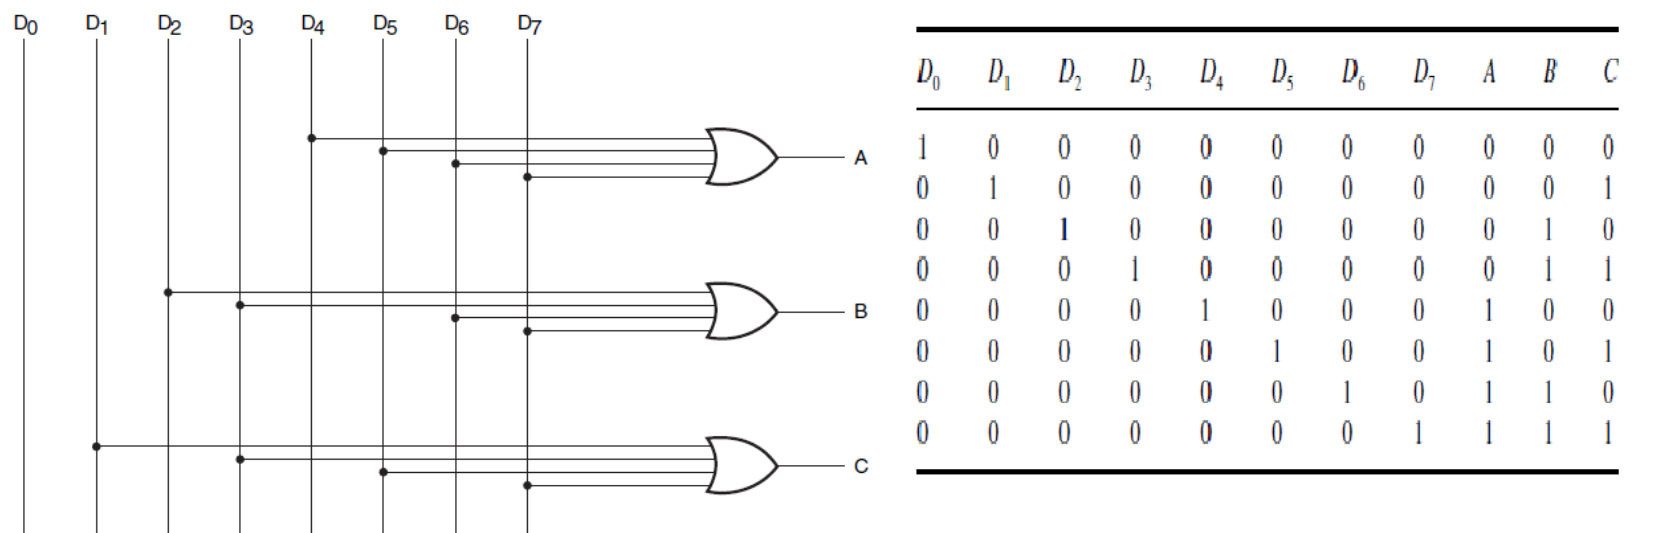
\includegraphics[width=0.9\textwidth]{encoder}
       	\end{frame}  	
    
    \section{Project 2}
    
    	\begin{frame}
         	\vfill
         	\centering
          	\begin{beamercolorbox}[sep=8pt,center,shadow=true,rounded=true]{title}
           	\usebeamerfont{title}Project 2\par%
        	\end{beamercolorbox}
            \vfill
       	\end{frame}

		\subsection{Project Tips}       	
       	
       	\begin{frame}
       		\frametitle{Project 2}
       		\begin{itemize}
       			\item For this project, you won't be working with decoders and encoders so much as you'll be working with adders.
       			\item We're moving on to the 'Arithmetic' portion of your ALU now (congrats, the logic processing is good to go!)
       			\item All you have to do now, is take care of how the ALU handles basic adding, and you should be set for this project
       			\item Remember the project guidelines and don't start too late!
       			\item As always, these slides and supplemental resources can be found on the course website
       		\end{itemize}
       	\end{frame}
		
		
    
    
\end{document}
